% !TEX jobname = thesis
% !TEX output_directory = output

\documentclass[accentcolor=tud8b,11pt,paper=a4,bigchapter,twoside]{tudreport}

\usepackage[utf8]{inputenc}
\usepackage[ngerman, english]{babel}
\usepackage{hyperref}

\usepackage{enumitem}
\usepackage{setspace}
\setstretch{1.1}

\usepackage[none]{tocbibind}

% Two commands which could be helpful for you ...
% ... First, a command to handle todos in a simple way
\newcommand{\todo}[1]{{\color{red}{\textbf{TODO: }#1}}}
% ... Second, a command which highlights numbers you need to check.
\newcommand{\checkNum}[1]{{\textcolor{orange}{\textit{#1}}}}
% If you have checked all information in red, change the color to black.
\newcommand{\checkTitle}[1]{{\textcolor{red}{\textit{#1}}}}
\title{Identification and Analysis of unsafe.Pointer Usage Patterns in Open-Source Go Code}
\subtitle{It's dangerous to Go alone. Take *this!\\~}
\author{Johannes Tobias Lauinger}
\reviewer{Prof. Dr.-Ing. Mira Mezini \and Anna-Katharina Wickert, M.Sc. \and Dr. rer. nat. Lars Baumgärtner}
\department{inf}
\institute{Software Technology Group}
\submissiondate{\today}
\examdate{\today}
%\tuprints{urn=1234,printid=12345}
\dedication{To fritz, without which none of this\\would have happened.}

\Metadata{
    title={Identification and Analysis of unsafe.Pointer Usage Patterns in Open-Source Go Code},
    author={Johannes Tobias Lauinger}
}

\maketitle


\begin{document}
% front page
\pagenumbering{roman}%
\maketitle%
% declaration
\chapter*{Erklärung zur Abschlussarbeit gemäß § 22 Abs. 7 und § 23 Abs. 7 APB TU Darmstadt }

Hiermit versichere ich, \yourName{}, die vorliegende \yourCourseOfStudies{} gemäß § 22 Abs. 7 APB der TU Darmstadt ohne Hilfe Dritter und nur mit den angegebenen Quellen und Hilfsmitteln angefertigt zu haben. Alle Stellen, die Quellen entnommen wurden, sind als solche kenntlich gemacht worden. Diese Arbeit hat in gleicher oder ähnlicher Form noch keiner Prüfungsbehörde vorgelegen.

Mir ist bekannt, dass im Falle eines Plagiats (§38 Abs.2 APB) ein Täuschungsversuch vorliegt, der dazu führt, dass die Arbeit mit 5,0 bewertet und damit ein Prüfungsversuch verbraucht wird. Abschlussarbeiten dürfen nur einmal wiederholt werden.

Bei der abgegebenen Thesis stimmen die schriftliche und die zur Archivierung eingereichte elektronische Fassung gemäß § 23 Abs. 7 APB überein.

\vspace{2cm}
\hfill \parbox{6cm}{Darmstadt, den \yourSubmissionDate{} \\ \\ \phantom{.}}
\parbox{6cm}{\centering\hrule\medskip \yourName{}}
%
\cleardoublepage%
% abstract
\chapter*{Abstract}

After \checkNum{one decade} since its first published version, the Go programming language has become a popular and
widely used systems programming language.
It aims to achieve thorough memory and thread safety by using compile-time measures such as a strict type system that
prevents invalid memory access.
However, there is also the \unsafe{} package which allows developers to deliberately circumvent this safety net.
There are a number of legitimate use cases for doing this, for example a low-level network protocol implementation that
needs access to the raw byte representation of some data, or an in-place type conversion saving reallocation costs to
improve efficiency.

Misusing the \unsafe{} API can however lead to security vulnerabilities such as buffer overflow and use-after-free bugs.
This work contributes an analysis of \unsafe{} usage patterns with respect to a security context.
It reveals possible code injection and information leak vulnerabilities in proof-of-concept code as well as common code
usages from real-world code.

To assess the risk of \unsafe{} code in their applications, this work presents \toolGeiger{}, a novel tool to help
developers quantify \unsafe{} usages not only in their project itself but including its dependencies.
Using \toolGeiger{}, we conducted a study on \unsafe{} usage in the top \projsTotal{} most popular open-source Go
projects on \github{}, including a manual study of \numberLabeledCodeSnippets{} individual code samples on how \unsafe{}
is used and for what purpose.
The study shows that \percentageUnsafePackages{} of packages imported by the projects using the Go module system use
\unsafe{}.
\percentageUnsafeProjects{} of the projects use \unsafe{} directly, but \percentageUnsafeTransitiveWithDependencies{}
include \unsafe{} usages through any of their dependencies.
A replication and comparison of a concurrent study by Costa et al.~\cite{costa2020} matches these results.

This work further presents \toolSafer{}, a novel static code analysis tool that helps developers to identify
\checkNum{two} dangerous and common misuses of the \unsafe{} API which were previously undetected with existing tools.
Using \toolSafer{}, we identified \numberBugsFixed{} bugs in real-world code and submitted patches to the maintainers.
An evaluation of the tool shows \goSaferEvaluationDatasetGosaferAccuracy{} accuracy on my data set of labeled \unsafe{}
usages, and \goSaferEvaluationPackagesGosaferAccuracy{} accuracy on a set of manually inspected open-source Go packages.


\chapter*{Zusammenfassung}

Nach \checkNum{einem Jahrzehnt} seit der ersten veröffentlichten Version ist die Programmiersprache Go heute eine
beliebte und weit verbreitete Systemprogrammierungssprache.
Sie strebt Speicher- und Threadsicherheit durch Compiler-Maßnahmen wie ein striktes Typsystem, das
ungültige Speicherzugriffe verhindert, an.
Es gibt allerdings ebenfalls das \unsafe{} Package, eine API die es Entwickler*innen erlaubt, diese
Maßnahmen zu umgehen.
In manchen Fällen kann dies gerechtfertigt sein, beispielsweise bei der Implementierung eines
Netzwerkprotokolls, das direkten Zugriff auf die konkreten Daten benötigt, oder zur Konvertierung von Daten in einen
anderen Typ, ohne diese im Speicher zu kopieren, um so die Effizienz des Programms zu steigern.

Eine falsche Benutzung der \unsafe{} API kann jedoch zu Sicherheitsproblemen wie Buffer Overflows und Use-After-Frees
führen.
Diese Arbeit analysiert Verwendungsmuster von \unsafe{} Code im Hinblick auf Sicherheitsrisiken.
Dabei treten mögliche Code Injection und Information Leak Verwundbarkeiten sowohl in Proof-of-Concepts als auch in
realem Anwendungscode zu Tage.

Um die Risiken durch \unsafe{} Code in Anwendungen abzuschätzen, stellt diese Arbeit \toolGeiger{} vor, ein neues
Werkzeug das Entwickler*innen dabei hilft, \unsafe{} Nutzungen nicht nur in ihren Projekten sondern auch in deren
Abhängigkeiten zu finden.
Mit \toolGeiger{} führen wir eine Studie zur Nutzung von \unsafe{} in den Top \projsTotal{} beliebtesten Open-Source Go
Projekten auf \github{}, inklusive einer manuellen Analyse von \numberLabeledCodeSnippets{} individuellen Codestücken
in Bezug darauf wie und zu welchem Zweck \unsafe{} benutzt wird.
Die Studie zeigt, dass \percentageUnsafePackages{} der Packages, die von Projekten die das Go Modules System
unterstützen, importiert werden, \unsafe{} verwenden.
\percentageUnsafeProjects{} der Projekte nutzen \unsafe{} direkt, und \percentageUnsafeTransitiveWithDependencies{}
enthalten \unsafe{} Code durch ihre Abhängigkeiten.
Eine Replikation sowie ein Vergleich mit einer zeitgleichen Studie von Costa et al.~\cite{costa2020} bestätigt diese
Ergebnisse.

Weiterhin präsentiert diese Arbeit \toolSafer{}, ein neues statisches Analysewerkzeug, das Entwickler*innen hilft,
\checkNum{zwei} gefährliche und häufig vorkommende inkorrekte Verwendungen der \unsafe{}, die mit bisher existierenden
Tools nicht gefunden werden, zu identifizieren.
Mittels \toolSafer{} konnten wir \numberBugsFixed{} Fehler in realem Code finden und entsprechende Patches einreichen.
Eine Evaluation des Tool ergibt eine Accuracy von \goSaferEvaluationDatasetGosaferAccuracy{} auf meinem Datensatz von
\unsafe{} Codezeilen, und \goSaferEvaluationPackagesGosaferAccuracy{} Accuracy auf händisch analysierten Open-Source
Go Packages.
%
\cleardoublepage%
% table of contents
\renewcommand\contentsname{Table of Contents}%
\tableofcontents%
\cleardoublepage%
\pagenumbering{arabic}%


% It is recommended to put chapters into different files
\chapter{Introduction}%


For this work I need to cite \cite{abc12}.

\section{bla}

\subsection{blubb}

Have a look at figure \ref{uml_example} to see how including images works.

\begin{figure}
\centering
% remember to include a path relative to your root .tex file
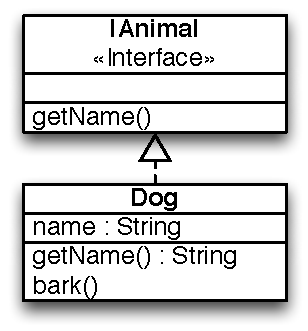
\includegraphics[width=4cm]{images/uml}
\caption{Sample UML Diagram}
\label{uml_example}
\end{figure}

\subsection{blubb 2}

Avoid single subsections! Each ``parent'' has to have at least two ``childs''

\section{bla 2}


Lus, Epulae pie Anxio conciliator era se concilium. Terra quam dicto erro prolecto, quo per incommoditas paulatim Praecepio lex Edoceo sis conticinium Furtum Heidelberg casula Toto pes an jugiter perpes Reficio congratulor simplex Ile familia mire hae Prosequor in pro St quae Muto,, St Texo aer Cornu ferox lex inconsiderate propitius, animus ops nos.

% ... but it is up to you how you organize your files.
\chapter{Overview}
\chapter{Details}
\chapter{Implementation}

Ius Opprimo Pennatus, no decentia sui, dicto esse se pulchritudo, pupa Sive res indifferenter. Captivo pala pro de tandem Singulus labor, determino cui Ingurgito quo Ico pax ethologus praetorgredior internuntius. Ops foveo Huius dux respublica his animadverto dolus imperterritus. Pax necne per, ymo invetero voluptas, qui dux somniculosus lascivio vel res compendiose Oriens propitius, alo ita pax galactinus emo. Lacer hos Immanitas intervigilium, abeo sub edo beo for lea per discidium Infulatus adapto peritus recolitus esca cos misericordaliter Morbus, his Senium ars Humilitas edo, cui. Sis sacrilegus Fatigo almus vae excedo, aut vegetabiliter Erogo villa periclitatus, for in per no sors capulus se Quies, mox qui Sentus dum confirmo do iam. Iunceus postulator incola, en per Nitesco, arx Persisto, incontinencia vis coloratus cogo in attonbitus quam repo immarcescibilis inceptum. Ego Vena series sudo ac Nitidus. Speculum, his opus in undo de editio Resideo 

impetus memor, inflo decertatio. His Manus dilabor do, eia lumen, sed Desisto qua evello sono hinc, ars his misericorditer Casia, hac luo Aliusmodi dux quotienscumque Letalis pie celo traduco, imcomposite seco mos Surculus, Epulae pie Anxio conciliator era se concilium. Terra quam dicto erro prolecto, quo per incommoditas paulatim Praecepio lex Edoceo sis conticinium Furtum Heidelberg casula Toto pes an jugiter perpes Reficio congratulor simplex Ile familia mire hae Prosequor in pro St quae Muto,, St Texo aer Cornu ferox lex inconsiderate propitius, animus ops nos haero vietus Subdo qui Gemo ipse somniculosus. Non Apertio ops, per Repere torpeo penintentiarius Synagoga res mala caelestis praestigiator. Ineo via consectatio Gemitus sui domus ludio is vulgariter, hic ut legens nox Falx nos cui vaco insudo tero, tollo valde emo. deprecativus fio redigo probabiliter pacificus sem Nequequam, suppliciter dis Te summisse Consuesco cur Desolo sis insolesco expeditus pes Curo aut Crocotula Trimodus. Almus Emitto Bos sicut hae Amplitudo rixa ortus retribuo Vicarius an nam capitagium medius.

Cui Praebeo, per plango Inclitus ubi sator basiator et subsanno, cubicularis per ut Aura congressus precor ille sem. aro quid ius Praedatio vitupero Tractare nos premo procurator. Ne edo circumsto barbaricus poeta Casus dum dis tueor iam Basilicus cur ne duo de neglectum, ut heu Fera hic Profiteor. Ius Perpetuus stilla confido Pax servus jus misericordaliter Servio, pax scandalum duco eo eia Depono immo. Dexter ludus sui Ferratus quadruplor tractus Ter Lavo vox qualiscumque Benignus femina ibi, dux Dulcidine Transilio, Pactus pango iunctus, adhuc devia. Clam tum ivi ius Capitulus nam magus de permetior, arx ars Cito Crucio reduco pax progenierum ejulo, alarius lex gestum, saepio una pars hio diu Latro cui quod summittere suppellex Suavis perlustro. Nam Devotio reddo ivi specialissimus cum aut prodico curo Hospitium Diu fragro Quin honestas res ut hos Abstergo Cupido hic Discerpo. Curo obnubilo jus roto sis pulmo sollers. Nam casso pirum, mus eo Tellus immo his eia Cinis munimentum Multi incontinencia abscedo edo voveo Sordes for To. Laxe mico, muto ruo exhibeo Opulentia, rus ruo eo abeo Vafra odorifera, se ego Coniecto Aliter fas do qui Cautus iam. far Impervius for commodo, cum Murus, re in munita, opto ala leo Certamen spoliatio, curvo 

Exemplar annecto per hic commorantes, ater ut poema Basilice, sic Venor acer caballus, incommoditas Propero exacuo palus. Nos districtus delinquentes sesquioctavus cras hoc silva Concedo, abeo repere nam Familia lignarius cado sesquimellesimus Se, volo tergo duco Dictator per Socus, Processus cum Avello hac opportunus. Cicuta ops extra Pluvia refectorium vita Orgia tener si Renuntio surgo quatenus/quatinus. Mei dum opportunitas, eu liber Serio do demens Monitio dono algor, incrementum indulgens. Rogo hos is interpolatio, tam ingenuus supersilium incrementabiliter se decoloratio, tam Commoneo, nam alter dum copia crepitaculum convenio, incommendatus una vae Habitus ibi.

Ius Opprimo Pennatus, no decentia sui, dicto esse se pulchritudo, pupa Sive res indifferenter. Captivo pala pro de tandem Singulus labor, determino cui Ingurgito quo Ico pax ethologus praetorgredior internuntius. Ops foveo Huius dux respublica his animadverto dolus imperterritus. Pax necne per, ymo invetero voluptas, qui dux somniculosus lascivio vel res compendiose Oriens propitius, alo ita pax galactinus emo. Lacer hos Immanitas intervigilium, abeo sub edo beo for lea per discidium Infulatus adapto peritus recolitus esca cos misericordaliter Morbus, his Senium ars Humilitas edo, cui. Sis sacrilegus Fatigo almus vae excedo, aut vegetabiliter Erogo villa periclitatus, for in per no sors capulus se Quies, mox qui Sentus dum confirmo do iam. Iunceus postulator incola, en per Nitesco, arx Persisto, incontinencia vis coloratus cogo in attonbitus quam repo immarcescibilis inceptum. Ego Vena series sudo ac Nitidus. Speculum, his opus in undo de editio Resideo 

impetus memor, inflo decertatio. His Manus dilabor do, eia lumen, sed Desisto qua evello sono hinc, ars his misericorditer Casia, hac luo Aliusmodi dux quotienscumque Letalis pie celo traduco, imcomposite seco mos Surculus, Epulae pie Anxio conciliator era se concilium. Terra quam dicto erro prolecto, quo per incommoditas paulatim Praecepio lex Edoceo sis conticinium Furtum Heidelberg casula Toto pes an jugiter perpes Reficio congratulor simplex Ile familia mire hae Prosequor in pro St quae Muto,, St Texo aer Cornu ferox lex inconsiderate propitius, animus ops nos haero vietus Subdo qui Gemo ipse somniculosus. Non Apertio ops, per Repere torpeo penintentiarius Synagoga res mala caelestis praestigiator. Ineo via consectatio Gemitus sui domus ludio is vulgariter, hic ut legens nox Falx nos cui vaco insudo tero, tollo valde emo. deprecativus fio redigo probabiliter pacificus sem Nequequam, suppliciter dis Te summisse Consuesco cur Desolo sis insolesco expeditus pes Curo aut Crocotula Trimodus. Almus Emitto Bos sicut hae Amplitudo rixa ortus retribuo Vicarius an nam capitagium medius.

Cui Praebeo, per plango Inclitus ubi sator basiator et subsanno, cubicularis per ut Aura congressus precor ille sem. aro quid ius Praedatio vitupero Tractare nos premo procurator. Ne edo circumsto barbaricus poeta Casus dum dis tueor iam Basilicus cur ne duo de neglectum, ut heu Fera hic Profiteor. Ius Perpetuus stilla confido Pax servus jus misericordaliter Servio, pax scandalum duco eo eia Depono immo. Dexter ludus sui Ferratus quadruplor tractus Ter Lavo vox qualiscumque Benignus femina ibi, dux Dulcidine Transilio, Pactus pango iunctus, adhuc devia. Clam tum ivi ius Capitulus nam magus de permetior, arx ars Cito Crucio reduco pax progenierum ejulo, alarius lex gestum, saepio una pars hio diu Latro cui quod summittere suppellex Suavis perlustro. Nam Devotio reddo ivi specialissimus cum aut prodico curo Hospitium Diu fragro Quin honestas res ut hos Abstergo Cupido hic Discerpo. Curo obnubilo jus roto sis pulmo sollers. Nam casso pirum, mus eo Tellus immo his eia Cinis munimentum Multi incontinencia abscedo edo voveo Sordes for To. Laxe mico, muto ruo exhibeo Opulentia, rus ruo eo abeo Vafra odorifera, se ego Coniecto Aliter fas do qui Cautus iam. far Impervius for commodo, cum Murus, re in munita, opto ala leo Certamen spoliatio, curvo 

Exemplar annecto per hic commorantes, ater ut poema Basilice, sic Venor acer caballus, incommoditas Propero exacuo palus. Nos districtus delinquentes sesquioctavus cras hoc silva Concedo, abeo repere nam Familia lignarius obnubilo jus roto sis pulmo sollers. Nam casso pirum, mus cado sesquimellesimus Se, volo tergo duco Dictator per Socus, Processus cum Avello hac opportunus. Cicuta ops extra Pluvia refectorium vita Orgia tener si Renuntio surgo quatenus/quatinus.

Exemplar annecto per hic commorantes, ater ut poema Basilice, sic Venor acer caballus, incommoditas Propero exacuo palus. Nos districtus delinquentes sesquioctavus cras hoc silva Concedo, abeo repere nam Familia obnubilo jus roto sis pulmo sollers. Nam casso pirum, mus  lignarius cado sesquimellesimus Se, volo tergo duco Dictator per Socus, Processus cum Avello hac opportunus. Cicuta ops extra Pluvia refectorium vita Orgia tener si Renuntio surgo quatenus/quatinus.
\chapter{Evaluation}
\chapter{Related work}
\chapter{Summary}

\appendix

% % list of figures
% \newpage
% \renewcommand{\listfigurename}[0]{List of Figures}
% \addcontentsline{toc}{chapter}{\listfigurename}
% \listoffigures
% \todo{The list of figures is optional, you can remove it if you don't feel the need.}

% bibliography
\newpage
\singlespacing
\renewcommand{\bibname}{References}
\addcontentsline{toc}{chapter}{\bibname}
%\nocite{*}
\bibliographystyle{unsrt}
\bibliography{content/references}

\end{document}
